
\chapter{TikZ gyorstalpaló}

\section{Alapok}

A \verb|\usepackage{tikzpicture}| kell a library implementálásához A \verb|\begin{tikzpicture}| és \verb|\end{tikzpicture}| parancsok közé kell helyezni a rajzolandó ábrát. A TikZ úgy működik, mint egy rajztábla. Egyesével kell az objektumokat rárajzolni, esetenként egy ciklusban többet is lehet egyszerre (lásd lejjebb). \textbf{Minden parancsot egy  ;-vel kell lezárni.}

A \verb|\begin{tikzpicture}["paraméterek"]| ebben a szögletes zárójelben kell megadni a rajztábla paramétereit. Ilyenek:
\begin{itemize}
    \item "\verb|scale = 3|"  -- a képet nyújtja, kivéve a betű méretet
    \item "\verb|xscale = 4, yscale = 5|"  -- ugyanez, csak merőlegesen affin képet ad
\end{itemize}

A rajzolásra két különböző, de általában mindenre elég parancs a \verb|\draw| és \verb|\filldraw| . A sima rajzolás csak körvonalat rajzol, a másik pedig automatikusan ugyanazzal a színnel kitölti az alakzatot. Mindkettő parancsnak meg kell mondani, hogy:

\begin{itemize}
    \item Hova: \verb|(x, y)|, \verb|(fok:hossz)|
    \item Mit: \verb|node|, \verb|--| (edge), \verb|circle|, \verb|rectangle|, \verb|arc|
    \item Stílusban: \verb|[color, ultra thin, fill]| -- ez lehet üres, ilyenkor a rajztábla stílusát használja
\end{itemize}

A node-ok kicsit trükkösebbek, róluk a gráfok részben lehet részletesebben olvasni.

\subsubsection{Kód}
\begin{SideBySideExample}
\begin{tikzpicture}[scale=3]
    %a köröknek a kp.-át és sugarát kell megadni
    \draw (0,0) circle (0.4 cm) [color = blue!90];
    \filldraw (1,0) circle (0.4 cm) [color = red!90];
    
    %a téglalapoknak a balalsó és jobbfelső csúcsait kell megadni
    \draw (2-0.4, -.4) rectangle (2+0.4, .4) [ultra thick, fill=black!20];
    
    %a törött vonalakat csúcsról csúcsra kell megadni
    \draw  (3-0.3, -0.3) -- (3-0.3, 0.4) -- (3+0.4, -0.4) -- (3+0.4, 0.4);
    
    %ami sokkal menőbb, például egy rácsbejáráshoz az íveltvonalak
    \draw[thick,rounded corners=8pt, color=pink!200] (4-0.3, -0.3) -- (4-0.3, 0.4) 
    -- (4+0.4, -0.4) -- (4+0.4, 0.4);
    
    %Ha a törött vonalat lezárnád érdemes a --cycle befejezést írni a kezdő csúcs 
    %megismétlése helyett.
\end{tikzpicture}
\end{SideBySideExample}

\subsubsection{Példa}
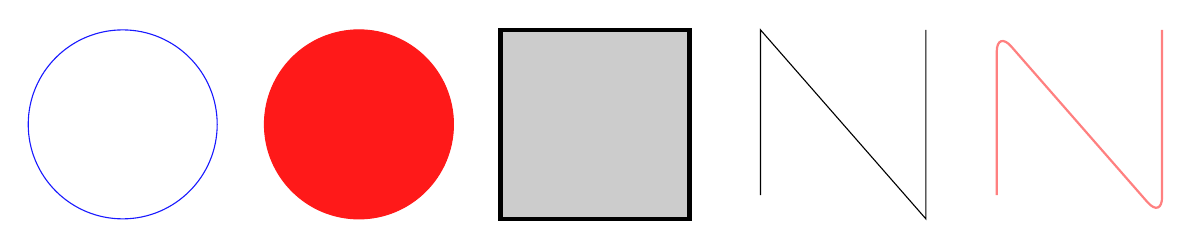
\begin{tikzpicture}[scale=3]
    %a köröknek a kp.-át és sugarát kell megadni
    \draw (0,0) circle (0.4 cm) [color = blue!90];
    \filldraw (1,0) circle (0.4 cm) [color = red!90];
    
    %a téglalapoknak a balalsó és jobbfelső csúcsait kell megadni
    \draw (2-0.4, -.4) rectangle (2+0.4, .4) [ultra thick, fill=black!20];
    
    %a törött vonalakat csúcsról csúcsra kell megadni
    \draw  (3-0.3, -0.3) -- (3-0.3, 0.4) -- (3+0.4, -0.4) -- (3+0.4, 0.4);
    
    %ami sokkal menőbb, például egy rácsbejáráshoz az íveltvonalak
    \draw[thick,rounded corners=8pt, color=pink!200] (4-0.3, -0.3) -- (4-0.3, 0.4) 
    -- (4+0.4, -0.4) -- (4+0.4, 0.4);
    
    %Ha a törött vonalat lezárnád érdemes a --cycle befejezést írni a kezdő csúcs %megismétlése helyett.
\end{tikzpicture}


\subsection{Illesztés}

Az első fejezetben leírtakat érdemes alkalmazni. A \verb|\clip| parancsot érdemes használni. Nem csak arra jó, hogy kivágjuk a kép egy részét, de beállítja a kép keretét, ha azzal kezdjük. Erre persze lehet használni a \verb|\useasboundingbox| parancsot amivel megadhatunk például egy téglalappal határolt fix keretét a képnek. Amit ezen kívül rajzoltál nem fogja megjeleníteni.

\subsubsection{Kód}
\selectlanguage{magyar}
\begin{Verbatim}

\begin{tikzpicture}[scale=3]        
    \draw (0,0) circle (0.4 cm) [color = blue!90];
    %Itt vágunk ami azt okozza, hogy az előző kör nem sérült
    \clip (-0.3, -0.3) rectangle (5, 0.3);
    \filldraw (1,0) circle (0.4 cm) [color = red!90];
    \draw (2-0.4, -.4) rectangle (2+0.4, .4) [ultra thick, fill=black!20];
    %Lehet relatív megadni a távolságokat, hogy ne kelljen mindent papíron kiszámolni
    %Ha csak sima +-t használsz, akkor a kezdő csúcstól viszonyít
    \draw  (3-0.3, -0.3) -- ++(0, 0.7) -- ++(0.7, -0.8) -- ++(0, 0.8);
    \draw[thick,rounded corners=8pt, color=pink!200]     (4-0.3, -0.3) -- (4-0.3, 0.4) -- (4+0.4, -0.4) -- (4+0.4, 0.4);
\end{tikzpicture}
\end{Verbatim}

\subsubsection{Példa}

\begin{tikzpicture}[scale=3]        
    \draw (0,0) circle (0.4 cm) [color = blue!90];
    %Itt vágunk ami azt okozza, hogy az előző kör nem sérült
    \clip (-0.3, -0.3) rectangle (5, 0.3);
    \filldraw (1,0) circle (0.4 cm) [color = red!90];
    \draw (2-0.4, -.4) rectangle (2+0.4, .4) [ultra thick, fill=black!20];
    %Lehet relatív megadni a távolságokat, hogy ne kelljen mindent papíron kiszámolni
    %Ha csak sima +-t használsz, akkor a kezdő csúcstól viszonyít
    \draw  (3-0.3, -0.3) -- ++(0, 0.7) -- ++(0.7, -0.8) -- ++(0, 0.8);
    \draw[thick,rounded corners=8pt, color=pink!200]     (4-0.3, -0.3) -- (4-0.3, 0.4) -- (4+0.4, -0.4) -- (4+0.4, 0.4);
\end{tikzpicture}

\subsection{Színek, egyebek}

Be lehet állítani vonalvastagságot, színt és még színátmenetes ábrát is egyszerű csinálni.
\begin{itemize}
    \item Vastagságok: \{\verb|ultra|, \verb|very|, \} + \{\verb|thin|, \verb|thick|\}
    \item Színek: \{ \verb|red|, \verb|green|, \verb|blue|, \verb|cyan|, \verb|magenta|, \verb|yellow|, \verb|black|, \verb|gray|, \verb|darkgray|, \verb|lightgray|, \verb|brown|, \verb|lime|, \verb|olive|, \verb|orange|, \verb|pink|, \verb|purple|, \verb|teal|, \verb|violet|, \verb|white| \}
    \item Vonal típusok: \{\verb|dashed|, \verb|dotted|\}
    \item Vonal összekötési lehetőségek (advanced): \begin{itemize}
        \item \verb|line cap = {round, rect, butt}|
        \item \verb|rounded corners = 5mm|
        \item \verb|line join = {round, bevel, mitern}|
        \end{itemize}
\end{itemize}

\subsubsection{Kód}
\selectlanguage{magyar}
\begin{Verbatim}
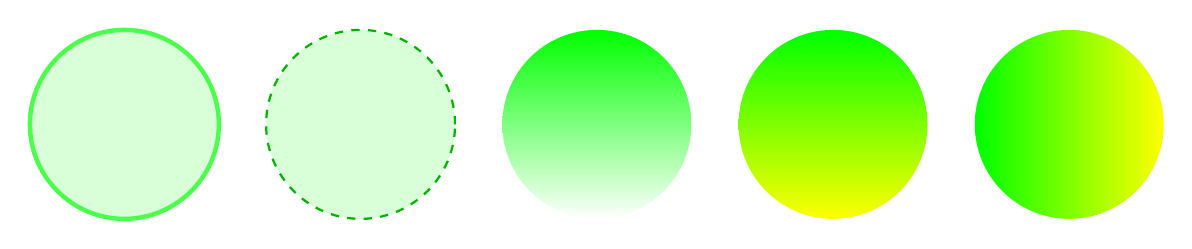
\begin{tikzpicture}[scale=3]
    \draw (0,0) circle (0.4) [color = green!70, fill = green!15, ultra thick];
    \draw (1,0) circle (0.4)     [color = green!70!black, fill = green!15, thick, dashed];
    \shade (2,0) circle (0.4) [top color = green];
    \shade (3,0) circle (0.4) [top color = green, bottom color = yellow];
    \shade (4,0) circle (0.4) [left color = green, right color = yellow];
\end{tikzpicture}
\end{Verbatim}

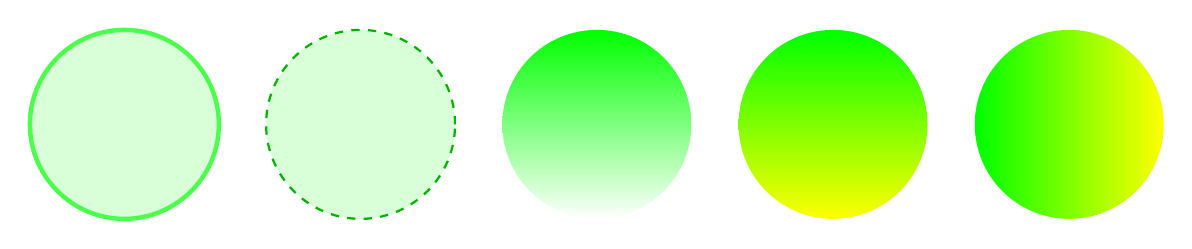
\begin{tikzpicture}[scale=3]
    \draw (0,0) circle (0.4) [color = green!70, fill = green!15, ultra thick];
    \draw (1,0) circle (0.4)     [color = green!70!black, fill = green!15, thick, dashed];
    \shade (2,0) circle (0.4) [top color = green];
    \shade (3,0) circle (0.4) [top color = green, bottom color = yellow];
    \shade (4,0) circle (0.4) [left color = green, right color = yellow];
\end{tikzpicture}

\section{Sokszögek rajzolása, for ciklusok}

Az, hogy lehet for ciklusokat írni, nagyban segít a valamilyen szempontból szimmetrikus ábrák elkészítésében. A for ciklusok hasonlóan más nyelvekhez bevezetnek egy változót, ami végig fut adott értékeken és végrehajtja a megadott parancsokat egyesével (jobb ha nem számít a sorrend).  Lehet egymásba ágyazott ciklusokat írni, de lehet párhuzamosan két vagy több változót egyszerre változtatni. Például \verb|\foreach \x in {1,2,3,4}{<commands>}| Ennél lehet komolyabb dolgokat is csinálni, lásd a példákat.

Eddig nem volt róla szó, de a hagyományos koordinátázás helyett lehet polárkoordinátákat is használni. \verb|(90:1cm)| -- 90 fok, 1 cm messze

A képet lehet transzformálni erre pár példa: \verb|xshift|, \verb|yshift|, \verb|rotate|

\subsubsection{Kód}
\selectlanguage{magyar}
\begin{Verbatim}
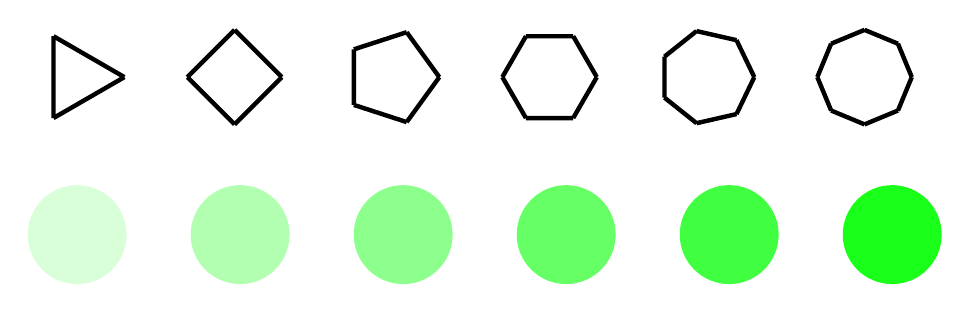
\begin{tikzpicture}[scale = 2, ultra thick]
    \foreach \n in {3, ..., 8}{    \draw (\n-3,0) \foreach \d in {1, ..., \n}{ %MAGIC DANGER        
            +(\d*360/\n:0.3cm) -- +(\d*360/\n + 360/\n:0.3cm)    }; 
            %Az, hogy ilyet lehet csinálni szerintem egyszerre undorító és hasznos
            %Ez kell ahhoz, hogy a szín mögé lehessen írni változót (nem igazán lehet képletet)
            \pgfmathsetmacro\i{\n*15-30} 
            \filldraw [xshift = \n-3, color = green!\i] (\n-3,-1) circle (0.3cm);
    }
\end{tikzpicture}
\end{Verbatim}

\subsubsection{Példa}
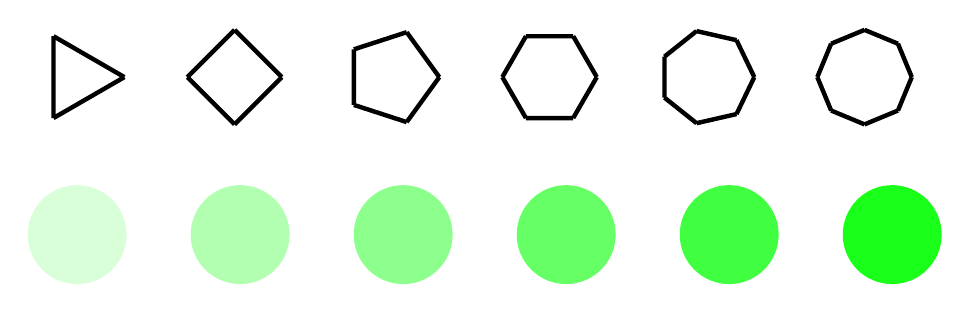
\begin{tikzpicture}[scale = 2, ultra thick]
    \foreach \n in {3, ..., 8}{    \draw (\n-3,0) \foreach \d in {1, ..., \n}{ %MAGIC DANGER        
            +(\d*360/\n:0.3cm) -- +(\d*360/\n + 360/\n:0.3cm)    }; 
            %Az, hogy ilyet lehet csinálni szerintem egyszerre undorító és hasznos
            %Ez kell ahhoz, hogy a szín mögé lehessen írni változót (nem igazán lehet képletet)
            \pgfmathsetmacro\i{\n*15-30} 
            \filldraw [xshift = \n-3, color = green!\i] (\n-3,-1) circle (0.3cm);
        }
\end{tikzpicture}

\section{Rácsok, szöveg beillesztése}

A \verb|\draw grid| parancsot lehet négyzetrács készítésre használni a \verb|\foreach| helyett. Meg kell adni a lépésközt és egy téglalapot ami határolja.

Szöveget beilleszteni úgy kell, hogy egy Node-ot töltünk fel szöveggel. Paraméterként meg lehet adni, hogy az adott pozícióhoz képest, hol helyezkedjen el a csúcs és így a szöveg, ezt az \verb|anchor=<direction>| paraméterrel lehet megadni. A \verb|fill=white| paraméter megadásával az is elérhető, hogy a szöveg/szám alatt megszakadjanak a vonalak, így egy sokkal esztétikusabb végeredményt kapunk. 
